\documentclass[a4paper,10pt]{article}

\usepackage{amssymb}
\usepackage{amsmath}
\usepackage{amstext}
\usepackage{amsthm}
\usepackage{esint} % more integral signs 
\usepackage{float}
\usepackage{graphicx}
\usepackage[margin=2.0cm]{geometry}
\usepackage{setspace}
\usepackage{url}

\setstretch{2.0}

\title{Multi-Domain Finite Element Meshing for Parotid Acinar Cell Modeling and Simulation}
\author{John Rugis$^{a,b}$ \and Nathan Pages$^b$ \and James Sneyd$^b$ \and David Yule$^c$}
\date{%
  $^a$corresponding author - email: j.rugis@auckland.ac.nz, phone: 649-373-7999\\%
  $^b$ Department of Mathematics,University of Auckland, Auckland, New Zealand\\%
  $^c$School of Medicine and Dentistry, University of Rochester, Rochester, NY, USA\\[2ex]%
  \today
}

\begin{document}
\maketitle

\newpage
\section*{Keywords}
multi-domain meshing, volumetric mesh, finite element modeling, parotid acinar cells.\\

\section*{Abstract}
350 words maximum.\\

\section{Introduction}
Double spaced. Wide margins.\\

\section{Introduction}

\section{Design Considerations}

\section{Description of Method}


\section{Results}
\begin{figure}[H]
\begin{center}
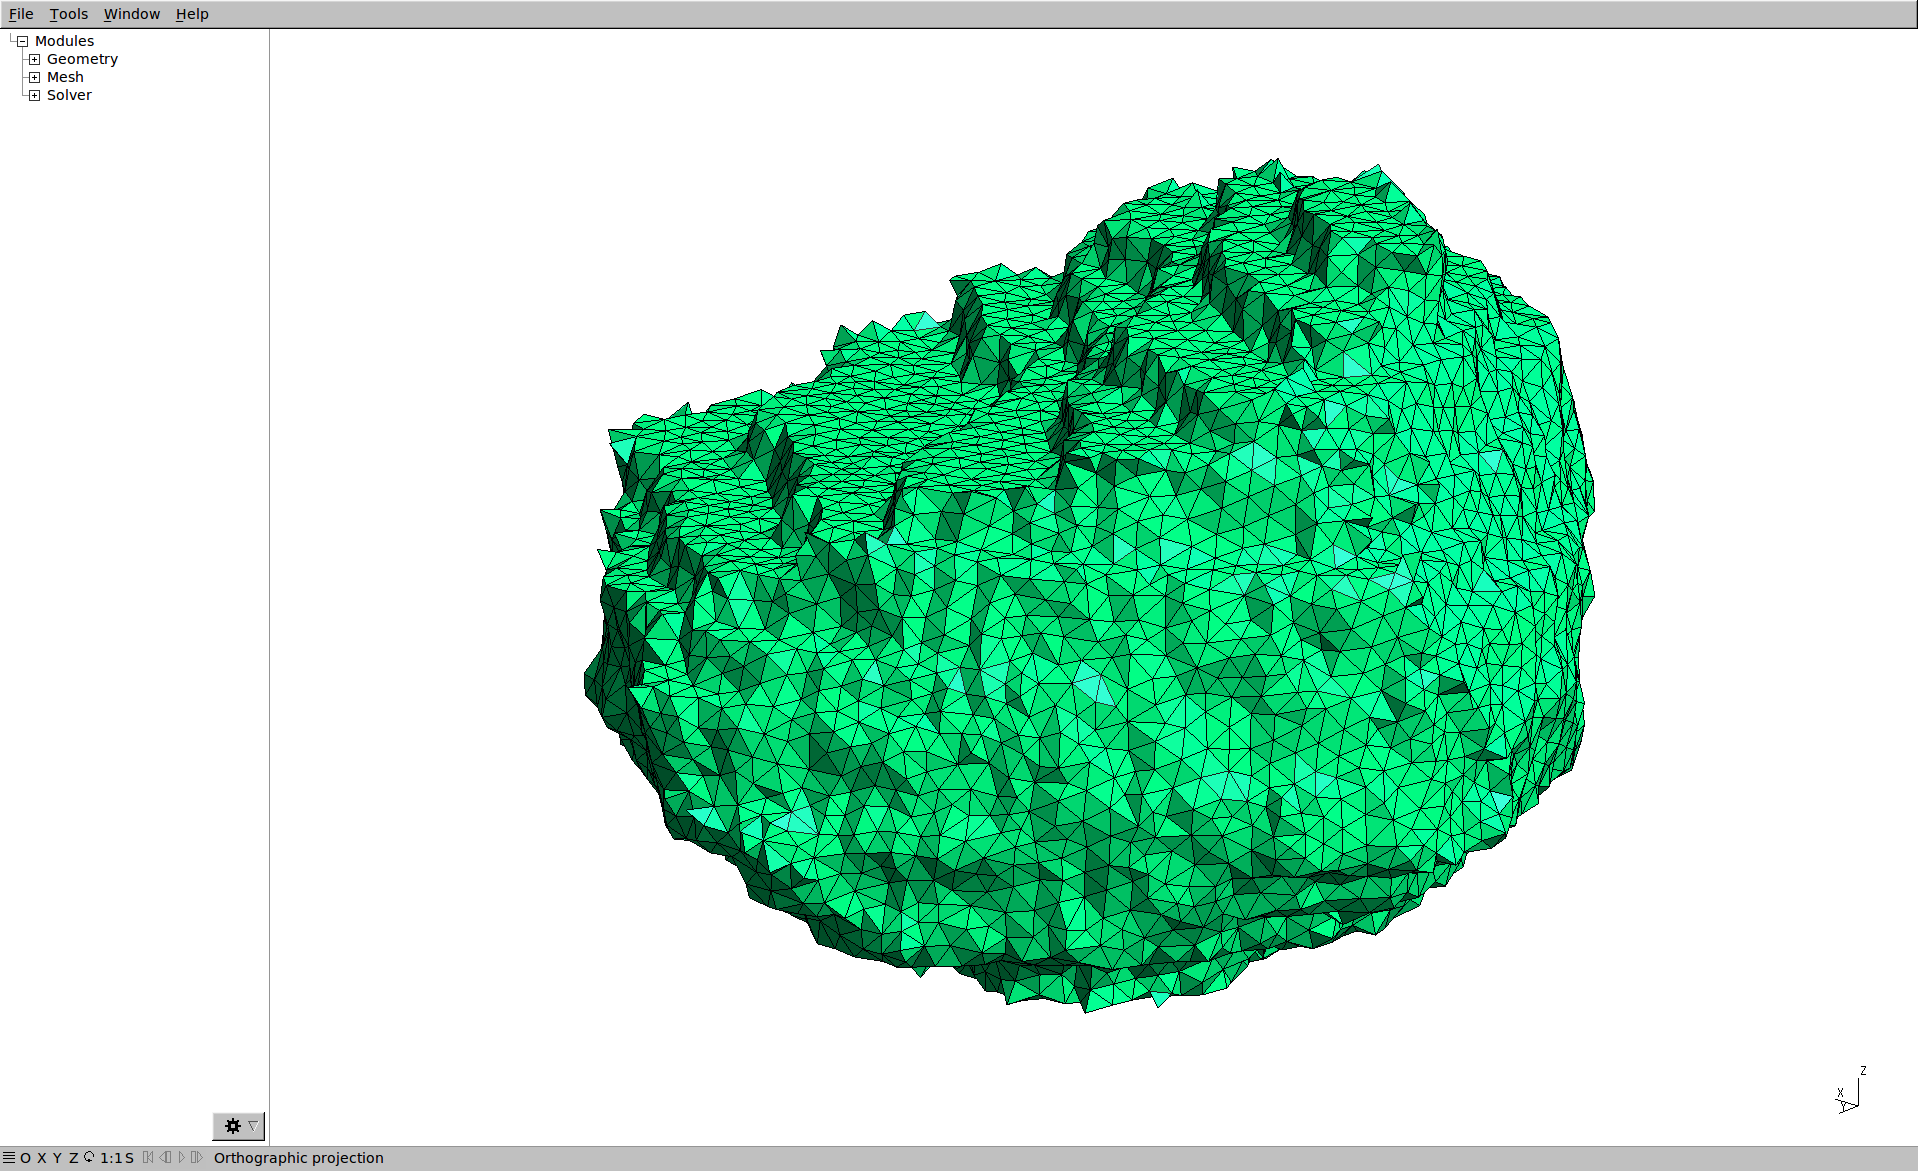
\includegraphics[width=0.45\textwidth]{images/cell1-00.png}
\end{center}
\end{figure}



\section{Discussion}

\section{Conclusion and Future Plans}

\section{Acknowledgements}
This work was supported by the National Institutes of Health grant number 5R01DE019245.\\

\section{References}

\end{document}